\section{Indicative Support Vector Clustering}
\subsection{Reweights of penalties}
\begin{frame}{Punishments are not fair}
Recall the penalty term...
\[
\min \left(R^2 + C\sum \xi_i\right)
\]
The higher the punishment value $C$ is...
\begin{itemize}
\item the lower the summation $\sum \xi_i$ is
\item the less likely $\xi_i > 0$
\item the less likely data points $\left\lbrace x_i\right\rbrace$ run out of sphere
\item the less outliers are allowed!
\end{itemize}
\pause
\vskip20pt 
\color{red} We see that, for all the outliers, penalty is the same $C$.
\end{frame}
\begin{frame}{Reweight the penalties}
Now we treat data points individually instead of equivalently penalizing all the input data with a constant $C$...
\begin{align}
\min \left(R^2 + \sum c_i\xi_i\right) \nonumber
\end{align}  
The larger the penalty $c_i$ is, the less possible the point $x_i$ would be driven away from the hypersphere, and vice versa. 
\pause
\vskip30pt
\begin{center}
\large
\color{blue} Full control over each point!
\end{center}
\end{frame}
\subsection{Integrate indicative information}
\begin{frame}{Assumption}
\begin{block}{ }
Anomalies are the patterns found to behave distinctly from the normal patterns, and similarly behaving instances are more likely hosted in the same cluster. 
\end{block}
\end{frame}
\begin{frame}{User given labels}
Suppose part of user feedback is available, 
\begin{center}
\begin{align*}
\mathcal{X^+}=&\left\lbrace \left( x_l, y_l) \,|\,  x_l \in \mathcal{X}, y_l=1 \right)\right\rbrace\\
\mathcal{X^-}=&\left\lbrace \left( x_r, y_r) \,|\, x_r \in \mathcal{X}, y_r=-1\right)\right\rbrace\\
&l, r \in \left\lbrace 1,\ldots ,N\right\rbrace
\end{align*}
\end{center}
$\mathcal{X^+}$ is set of outliers indicated by users, and $\mathcal{X}$ a set of normal samples.
\end{frame}
\begin{frame}{Impact function}
The closer to the indicated data, the more likely they belong to the same set (normal/outlier)
\begin{figure}
\centering
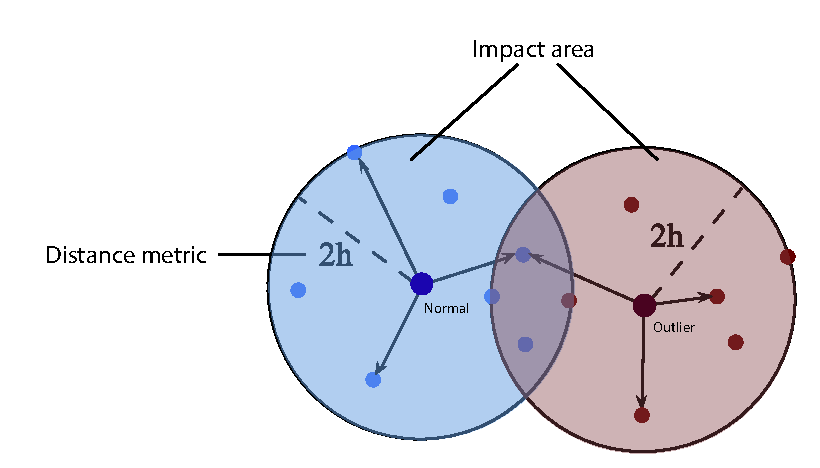
\includegraphics[scale=0.5]{imgs/indicative2.pdf}
\end{figure}
\vskip10pt
\pause
\color{blue}So, the penalties can be reweighed by distances to the given labeled data points.
\end{frame}

\subsection{Observations}
\begin{frame}{We observed}
Points near the given outliers $\mathcal{X^+}$
\begin{itemize}
\item Penalties $c_j$ are small
\item More likely to be repelled
\item Impact on cluster center $g$ is small
\end{itemize}
\pause
Points near the given normals $\mathcal{X^-}$
\begin{itemize}
\item Penalties $c_j$ are big
\item More likely to be enclosed into the ball
\item Impact on cluster center $g$ is larger
\end{itemize}
\pause
Leads to...
\begin{itemize}
\item Robustness
\item Reliable outlier detection
\item Better clustering results
\item More compact bound
\end{itemize}
\end{frame}
%\begin{frame}{Statistical Implication}
%\begin{block}{Reichenbach's \textit{Common Cause Principle}}
%If $X$ and $Y$ are correlated, then either $X$ causes $Y$ or $Y$ causes $X$ or they share a latent common cause $Z$.
%\end{block}
%\begin{figure}
%\setcounter{subfigure}{0}
%	\centering
%	\begin{subfigure}[H]{0.3\textwidth}
%		\centering
%		\includegraphics[scale=0.3]{imgs/x2y}
%		\caption{$X$ causes $Y$}
%		%\label{}	
%	\end{subfigure}
%	\begin{subfigure}[H]{0.3\textwidth}
%		\centering
%		\includegraphics[scale=0.3]{imgs/y2x}
%		\caption{$Y$ causes $X$}
%		%\label{}	
%	\end{subfigure}
%	\begin{subfigure}[H]{0.3\textwidth}
%		\centering
%		\includegraphics[scale=0.3]{imgs/z2xy}
%		\caption{A common latent cause $Z$}
%		%\label{}	
%	\end{subfigure}
%\end{figure}\pause
%\begin{itemize}
%\item<+-|alert@+> It links causality with probability
%\end{itemize}
%\end{frame}
%\begin{frame}{Functional Causal Model (pearl et al.)} 
%\begin{itemize}[<+->]
%\item A set of variables (factors) $\left\lbrace X_1,\ldots,X_n \right\rbrace$
%\item Directed acyclic graph $\mathcal{G}$ with vertices $\left\lbrace X_1,\ldots,X_n \right\rbrace$
%\item Parents of node $X_i$ in $\mathcal{G}$ are its direct causes
%\item $X_i=f_i(Parents(X_i),\epsilon_i)$, where $\left\lbrace\epsilon_1,\ldots,\epsilon_n\right\rbrace$ are jointly independent noises
%\item The above entails a joint probability distribution $P(X_1,\ldots,X_n)$
%\item Problems are twofold:
%      \begin{enumerate}
%		\item How is the $P$ like?
%		\item Can we recover $\mathcal{G} from P$? 
%	\end{enumerate}
%\item[] \begin{textblock*}{200mm}(0.6\textwidth,-2cm)
%		\includegraphics[scale=0.25]{imgs/causalgm}
%	\end{textblock*}
%\end{itemize}
%\end{frame}
%\begin{frame}{Functional Causal Model, ctd.}
%The following are equivalent:
%\begin{itemize}
%\item A functional causal model exists
%\item Local causal Markov condition: $X_i$ is statistically independent of its non-descendants given $X_i$'s parents
%\item Global Causal Markov condition: \textbf{d-separation} characterize the set of independences over all the observables
%\item Factorization: $P(X_1,\ldots,X_n)=\prod_iP(X_i\,|\,Parents(X_i))$
%\end{itemize}
%\end{frame}
%\begin{frame}{Learning causation from Data?}
%\begin{block}{Question}
%Given observational data, can we infer $\mathcal{G}$?
%\end{block}
%\begin{itemize}
%\item \textbf{Simple answer:} impossible without additional information
%\item Possible with interventions (outside force, empirical treatment, etc.)
%\item By conditional independence tests, \textit{Markov equivalence class} containing $\mathcal{G}$ can be learned. \alert{But}, it fails in simplest 2-nodes case.
%\item 2-nodes case can be tackled applying residual dependence test. (see Hoyer et al.)
%\end{itemize}
%\end{frame}
%\begin{frame}{Markov Equivalence Class}
%\textbf{Simplest case with three variables}
%\begin{itemize}
%\item[]<1-> \begin{figure}
%\setcounter{subfigure}{0}
%			\begin{subfigure}[H]{0.4\textwidth}
%			\includegraphics[scale=0.4]{imgs/eqv}
%			\caption{Equivalence}
%			\end{subfigure}\hfill
%			\begin{subfigure}[H]{0.3\textwidth}
%			\includegraphics[scale=0.4]{imgs/noneqv}
%			\caption{Non-equivalence}
%			\end{subfigure}
%		\end{figure}
%\item<2-> Samples can be explained by all graphs in equivalence class
%\item<3-> For example:
%\begin{table}
%\centering
%\begin{tabular}{|c|c|}
%\hline
%Equivalence class & Non-equivalence class \\\hline
%$Dep(X,Z\,|\,\emptyset)$ & $Dep(X,Z\,|\,\emptyset)$\\\hline
%$Dep(Y,Z\,|\,\emptyset)$ & $Dep(Y,Z\,|\,\emptyset)$\\\hline
%$Dep(X,Y\,|\,\emptyset)$ & \alert{$Ind(X,Y\,|\,\emptyset)$}\\\hline
%$Ind(X,Y\,|\,Z)$ & \alert{$Dep(X,Y\,|\,Z)$}\\\hline
%\end{tabular}
%\end{table}	
%\end{itemize}
%\end{frame}